\chapter{Voortplanting van signalen: lopende en staande golven}\label{ch:b1:wave-propagation}

Tokkel een gitaarsnaar aan en een hele zaal hoort een toon; leg een vinger
licht op het midden en de toon springt een octaaf omhoog. Ga tussen twee
luidsprekers staan die dezelfde toon spelen en je passeert al wandelend om de
paar decimeter een plek van bijna volledige stilte. Licht uit twee gaatjes
schildert strepen op een scherm. In geen van deze gevallen wordt er iets van de
ene plaats naar de andere gedragen --- geen lucht, geen snaar, geen glas
verplaatst zich --- en toch plant zich iets voort: een \emph{\omterm{def:b1:wave-propagation:signal}{signaal}}. Dit
hoofdstuk beschrijft hoe een \omterm{def:b1:wave-propagation:signal}{signaal} zich verplaatst, wat een sinusvormige golf
is en wat er gebeurt wanneer twee golven elkaar ontmoeten: de wiskunde van
superpositie, interferentie en staande golven, die elk later golfhoofdstuk ---
akoestiek, optica en kwantumfysica --- opnieuw gebruikt.

\begin{omfigure}
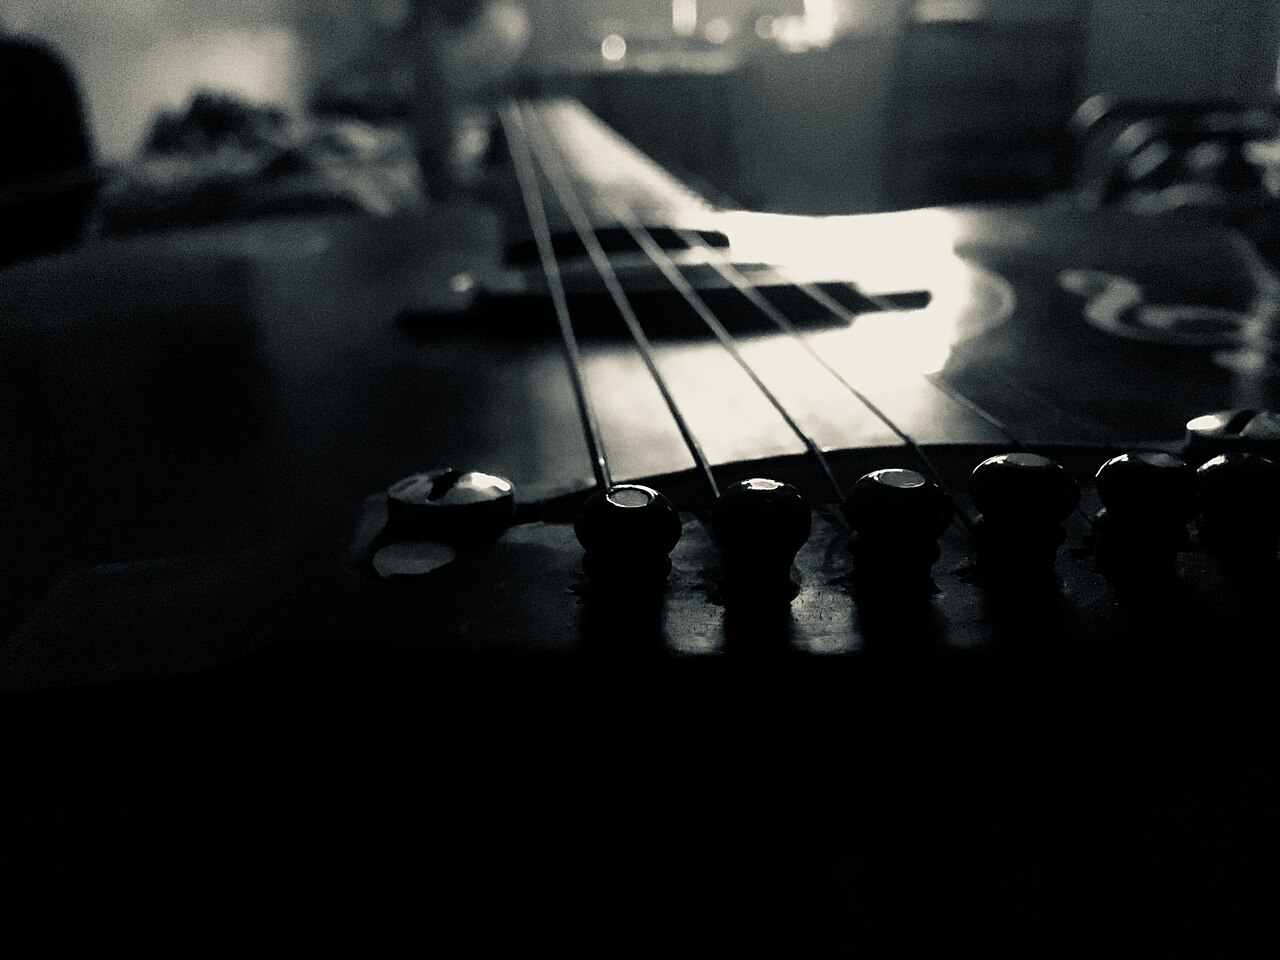
\includegraphics[width=0.55\linewidth]{images/book3/guitar-closeup.jpg}

{\small Zes snaren, zes grondfrequenties: elke snaar is een \omterm{thm:b1:wave-propagation:standing}{staande golf} die aan de topkam en de kam is vastgelegd, en de vingers verkorten haar om de toonhoogte te verhogen.}
\end{omfigure}

\section{Signalen}

\begin{definition}[Signaal; sinusvormig signaal]\label{def:b1:wave-propagation:signal}
\index{signaal}\index{sinusvormig signaal}\index{amplitude}\index{fase}\index{hoekfrequentie}
Een \emph{signaal} is een \omterm{def:b1:units-dimensions:unit}{natuurkundige grootheid} die in de tijd verandert en
informatie draagt: de akoestische overdruk aan een microfoon, de spanning aan
een antenne, de dwarsuitwijking van een punt van een snaar. Het
\emph{sinusvormige signaal}
\[
s(t) = A\cos(\omega t + \varphi)
\]
heeft \emph{amplitude} $A > 0$, \emph{hoekfrequentie} $\omega$
(\unit{rad/s}), \emph{frequentie} $f = \omega/2\pi$, \emph{periode}
$T = 1/f$ en \emph{beginfase} $\varphi$; $\omega t + \varphi$ is
zijn \emph{fase} op tijdstip $t$.
\end{definition}

\begin{remark}[Spectrum]\label{rem:b1:wave-propagation:spectrum}
\index{spectrum!van een signaal}\index{harmonische}
Elk periodiek \omterm{def:b1:wave-propagation:signal}{signaal} met periode $T$ is een som van sinussen met frequenties
$f_1 = 1/T$ (de \emph{grondtoon}) en veelvouden $nf_1$ daarvan (de
\emph{harmonischen}); de lijst van hun \omterm{def:b1:wave-propagation:signal}{amplitudes} is het \emph{spectrum} van
het \omterm{def:b1:wave-propagation:signal}{signaal}. Een fluit en een viool die dezelfde noot spelen delen de
grondtoon en verschillen in spectrum --- dat is klankkleur. De ontbinding
(die van Fourier) wordt geformuleerd en gebruikt in
\cref{ch:b1:filters-transfer-functions}; hier telt zij omdat sinussen zich
eenvoudig voortplanten, en wat voor elke sinus geldt, geldt door optelling
voor elk \omterm{def:b1:wave-propagation:signal}{signaal}.
\end{remark}

\begin{proposition}[Zwevingen]\label{prop:b1:wave-propagation:beats}
\index{zwevingen}
De som van twee sinussen met gelijke \omterm{def:b1:wave-propagation:signal}{amplitude} en nabije frequenties
$f_1 > f_2$,
\[
A\cos(2\pi f_1 t) + A\cos(2\pi f_2 t)
= 2A\cos\!\big(2\pi\tfrac{f_1 - f_2}{2}\,t\big)\cos\!\big(2\pi\tfrac{f_1 + f_2}{2}\,t\big),
\]
is een sinus met de gemiddelde frequentie waarvan de \omterm{def:b1:wave-propagation:signal}{amplitude}
$\abs{2A\cos(\pi(f_1 - f_2)t)}$ aanzwelt en wegebt met de
\emph{zwevingsfrequentie} $f_1 - f_2$.
\end{proposition}

\begin{proof}
$\cos a + \cos b = 2\cos\frac{a - b}{2}\cos\frac{a + b}{2}$. De trage
factor wordt twee keer nul per eigen periode $2/(f_1 - f_2)$, zodat de
omhullende $\abs{\cdot}$ frequentie $f_1 - f_2$ heeft.
\end{proof}

\begin{omfigure}
\begin{tikzpicture}
\begin{axis}[omaxis, axis x line=bottom, width=11.5cm, height=4.6cm, xlabel={$t$ (\unit{s})},
    ylabel={$s$}, xmin=0, xmax=1, ymin=-2.3, ymax=2.3, ytick={-2,0,2},
    yticklabels={$-2A$,$0$,$2A$}, xtick={0,0.25,0.5,0.75,1}]
  \addplot[omDef, thick, domain=0:1, samples=700] {cos(deg(2*pi*22*x)) + cos(deg(2*pi*20*x))};
  \addplot[omThm, thick, dashed, domain=0:1, samples=200] {2*cos(deg(2*pi*1*x))};
  \addplot[omThm, thick, dashed, domain=0:1, samples=200] {-2*cos(deg(2*pi*1*x))};
\end{axis}
\end{tikzpicture}

{\small Zwevingen tussen \qty{22}{Hz} en \qty{20}{Hz}: een trilling van
\qty{21}{Hz} waarvan de omhullende (streepjes) twee keer per seconde zweeft ---
het verschil van de frequenties.}
\end{omfigure}

\begin{example}[Op het gehoor stemmen]\label{ex:b1:wave-propagation:tuning}
Een stemvork van \qty{440}{Hz} en een snaar van \qty{443}{Hz} die samen
klinken bonzen drie keer per seconde; de snaar aanspannen vertraagt het
bonzen, en als het ophoudt is de snaar zuiver. Het oor hoort de gemiddelde
frequentie (\qty{441.5}{Hz}) als toonhoogte en de omhullende van \qty{3}{Hz}
als schommelende luidheid: zwevingen maken een frequentieverschil van minder
dan een procent hoorbaar.
\end{example}

\section{Lopende golven}

\begin{definition}[Lopende golf, voortplantingssnelheid]\label{def:b1:wave-propagation:travelling}
\index{lopende golf}\index{voortplantingssnelheid}\index{niet-dispersief medium}
Een \omterm{def:b1:wave-propagation:signal}{signaal} $s(x, t)$ dat langs een as is gedefinieerd is een \emph{lopende
golf} die zich in de richting $+x$ verplaatst met \emph{voortplantingssnelheid} $c$ als
\[
s(x, t) = f\!\left(t - \frac{x}{c}\right) = F(x - ct)
\]
voor een zekere functie $f$ (of $F$): de vorm wordt onvervormd meegevoerd,
over $c\,\Delta t$ verschoven in de tijd $\Delta t$. Een golf die naar $-x$ loopt is
$g(t + x/c)$. Een medium waarin elke vorm zich onvervormd voortplant met
dezelfde $c$ heet \emph{niet-dispersief}.
\end{definition}

\begin{proposition}[Vertraging]\label{prop:b1:wave-propagation:delay}
Het \omterm{def:b1:wave-propagation:signal}{signaal} dat in $x_2$ wordt ontvangen is het \omterm{def:b1:wave-propagation:signal}{signaal} dat in $x_1 < x_2$ is
uitgezonden, vertraagd over $\tau = (x_2 - x_1)/c$: $s(x_2, t) = s(x_1, t - \tau)$.
\end{proposition}

\begin{proof}
$s(x_2, t) = f(t - x_2/c) = f\big((t - \tau) - x_1/c\big) = s(x_1, t - \tau)$.
\end{proof}

\begin{example}[Voortplantingssnelheden]\label{ex:b1:wave-propagation:celerities}
Geluid in lucht, \qty{340}{m/s}: donder \qty{3}{s} na de flits legt de
inslag \qty{1}{km} verderop. Geluid in water, \qty{1500}{m/s}; in staal,
\qty{5000}{m/s}. Dwarsgolven op een snaar met spankracht $F$ en massa
per lengte-eenheid $\mu$: $c = \sqrt{F/\mu}$, zoals de dimensieanalyse
voorspelde (\cref{exo:b1:units-dimensions:5}) --- \qty{140}{m/s} voor een
gitaarsnaar. Licht in vacuüm, $c = \qty{3.00e8}{m/s}$; in glas,
$c/n$. De \omterm{def:b1:wave-propagation:travelling}{voortplantingssnelheid} is een eigenschap van het medium, niet van
de bron: een gefluister en een schreeuw komen samen aan.
\end{example}

\begin{proposition}[Sinusvormige lopende golf]\label{prop:b1:wave-propagation:sinusoidal}
\index{golflengte}\index{golfgetal}\index{fasesnelheid}\index{dubbele periodiciteit}
Een sinusvormige bron $s(0, t) = A\cos(\omega t)$ zendt uit
\[
s(x, t) = A\cos\!\big(\omega(t - x/c)\big) = A\cos(\omega t - kx),
\qquad k = \frac{\omega}{c} = \frac{2\pi}{\lambda},
\qquad \lambda = cT = \frac{c}{f}.
\]
De golf is periodiek in de tijd (periode $T$) en in de ruimte (periode de
\emph{golflengte} $\lambda$); $k$ is het \emph{golfgetal}; twee punten
op afstand $d$ trillen met een faseverschil
$\Delta\varphi = 2\pi d/\lambda = kd$ --- in \omterm{def:b1:wave-propagation:signal}{fase} als $d = n\lambda$, in
tegenfase als $d = (n + \tfrac12)\lambda$. De snelheid waarmee een
golftop zich verplaatst, $v_\varphi = \omega/k$, is de \emph{fasesnelheid};
hier is $v_\varphi = c$.
\end{proposition}

\begin{proof}
Vul $f(u) = A\cos(\omega u)$ in $f(t - x/c)$ in. Bij vaste $x$ herhaalt het
\omterm{def:b1:wave-propagation:signal}{signaal} zich na $T = 2\pi/\omega$; bij vaste $t$ herhaalt het zich na
$\lambda$ met $k\lambda = 2\pi$. Twee punten $x_1$, $x_2 = x_1 + d$: hun
\omterm{def:b1:wave-propagation:signal}{fasen} verschillen $kd$. Een golftop ($\omega t - kx = \text{const}$) beweegt met
$\dd x/\dd t = \omega/k$.
\end{proof}

\begin{omfigure}
\begin{tikzpicture}
\begin{axis}[omaxis, width=7.2cm, height=4.2cm, xlabel={$x$}, ylabel={$s(x, t_0)$},
    xmin=0, xmax=6.5, ymin=-1.4, ymax=1.6, ytick={-1,0,1}, yticklabels={$-A$,$0$,$A$},
    xtick={0,2,4,6}, xticklabels={$0$,$\lambda$,$2\lambda$,$3\lambda$}]
  \addplot[omDef, thick, domain=0:6.5, samples=200] {cos(deg(pi*x))};
  \draw[Stealth-Stealth, omThm] (axis cs:2,1.2) -- (axis cs:4,1.2) node[midway, above, font=\footnotesize] {$\lambda$};
  \draw[-Stealth, omExo, thick] (axis cs:4.7,1.2) -- (axis cs:5.7,1.2) node[midway, above, font=\footnotesize] {$c$};
\end{axis}
\end{tikzpicture}\qquad
\begin{tikzpicture}
\begin{axis}[omaxis, width=7.2cm, height=4.2cm, xlabel={$t$}, ylabel={$s(x_0, t)$},
    xmin=0, xmax=6.5, ymin=-1.4, ymax=1.6, ytick={-1,0,1}, yticklabels={$-A$,$0$,$A$},
    xtick={0,2,4,6}, xticklabels={$0$,$T$,$2T$,$3T$}]
  \addplot[omDef, thick, domain=0:6.5, samples=200] {cos(deg(pi*x))};
  \draw[Stealth-Stealth, omThm] (axis cs:2,1.2) -- (axis cs:4,1.2) node[midway, above, font=\footnotesize] {$T$};
\end{axis}
\end{tikzpicture}

{\small De \omterm{prop:b1:wave-propagation:sinusoidal}{dubbele periodiciteit} van een sinusvormige \omterm{def:b1:wave-propagation:travelling}{lopende golf}: een
momentopname bij vaste tijd herhaalt zich elke golflengte $\lambda$ en schuift
op met snelheid $c$; het \omterm{def:b1:wave-propagation:signal}{signaal} in een vast punt herhaalt zich elke periode
$T$, met $\lambda = cT$.}
\end{omfigure}

\begin{definition}[Dispersie]\label{def:b1:wave-propagation:dispersion}
\index{dispersief medium}
Een medium is \emph{dispersief} wanneer de fasesnelheid van de frequentie
afhangt. Een niet-sinusvormig \omterm{def:b1:wave-propagation:signal}{signaal}, een som van sinussen, vervormt dan
onderweg doordat zijn componenten uit elkaar lopen. Geluid in lucht en licht in
vacuüm zijn niet-dispersief; licht in glas (\cref{ch:b1:rays-reflection-refraction})
en golven op diep water zijn dispersief --- de lange deining van een verre
storm komt een dag eerder aan dan de korte kabbeling.
\end{definition}

\section{Superpositie en interferentie}

\begin{theorem}[Superpositie]\label{thm:b1:wave-propagation:superposition}
\index{superpositiebeginsel}
Planten in een lineair medium meerdere golven zich samen voort, dan is het
resulterende \omterm{def:b1:wave-propagation:signal}{signaal} op elke plaats en elk tijdstip de som van de signalen die
elke golf alleen zou opwekken.
\end{theorem}
\admitted

\begin{remark}[Lineariteit]\label{rem:b1:wave-propagation:linearity}
Superpositie is een uitspraak over de vergelijkingen van het medium (lineair
in het \omterm{def:b1:wave-propagation:signal}{signaal}), waar zolang de \omterm{def:b1:wave-propagation:signal}{amplitudes} klein blijven: geluid onder de
pijngrens, licht onder de intensiteit van een snijlaser, een zacht getokkelde
snaar. Twee lichtbundels kruisen elkaar zonder elkaar te storen; twee rimpels
gaan door elkaar heen en komen er ongeschonden uit. Wat men \emph{waarneemt
waar zij elkaar overlappen} is het onderwerp van de interferentie.
\end{remark}

\begin{theorem}[Twee sinusvormige signalen van dezelfde frequentie]\label{thm:b1:wave-propagation:fresnel}
\index{interferentie}\index{formule van Fresnel}\index{constructieve interferentie}\index{destructieve interferentie}
In een punt waar twee sinusvormige signalen van dezelfde frequentie aankomen,
$s_1 = A_1\cos(\omega t + \varphi_1)$ en $s_2 = A_2\cos(\omega t + \varphi_2)$,
is de som een sinus met dezelfde frequentie waarvan de \omterm{def:b1:wave-propagation:signal}{amplitude} voldoet aan
\[
A^2 = A_1^2 + A_2^2 + 2A_1A_2\cos\Delta\varphi,
\qquad \Delta\varphi = \varphi_2 - \varphi_1 .
\]
Voor golven waarvan de intensiteit (vermogen per oppervlakte) evenredig is met
$A^2$ voldoen de intensiteiten aan de \emph{formule van Fresnel}
\[
I = I_1 + I_2 + 2\sqrt{I_1 I_2}\,\cos\Delta\varphi .
\]
De interferentie is \emph{constructief} ($A = A_1 + A_2$) wanneer
$\Delta\varphi = 2n\pi$, en \emph{destructief} ($A = \abs{A_1 - A_2}$)
wanneer $\Delta\varphi = (2n + 1)\pi$, $n \in \Z$.
\end{theorem}

\begin{proof}
Uitwerken: $s_1 + s_2 = (A_1\cos\varphi_1 + A_2\cos\varphi_2)\cos\omega t -
(A_1\sin\varphi_1 + A_2\sin\varphi_2)\sin\omega t = X\cos\omega t -
Y\sin\omega t = A\cos(\omega t + \varphi)$ met $A^2 = X^2 + Y^2 =
A_1^2 + A_2^2 + 2A_1A_2(\cos\varphi_1\cos\varphi_2 + \sin\varphi_1\sin\varphi_2)$.
Meetkundig: $A$ is de lengte van de som van twee vectoren met lengtes
$A_1$, $A_2$ die de hoek $\Delta\varphi$ maken (de cosinusregel).
\end{proof}

\begin{proposition}[Twee bronnen in fase; wegverschil]\label{prop:b1:wave-propagation:pathdiff}
\index{wegverschil}
Twee bronnen die in \omterm{def:b1:wave-propagation:signal}{fase} uitzenden met golflengte $\lambda$, op afstanden
$d_1$ en $d_2$ van een punt $M$, komen in $M$ aan met
$\Delta\varphi = 2\pi\,\delta/\lambda$, waarin $\delta = d_2 - d_1$ het
\emph{\omterm{prop:b1:wave-propagation:pathdiff}{wegverschil}} is. De interferentie in $M$ is constructief als
$\delta = n\lambda$, destructief als $\delta = (n + \tfrac12)\lambda$.
\end{proposition}

\begin{proof}
Elke golf komt aan met de faseachterstand $kd_i = 2\pi d_i/\lambda$ van haar
reis (\cref{prop:b1:wave-propagation:sinusoidal}); het verschil is
$2\pi(d_2 - d_1)/\lambda$. Pas \cref{thm:b1:wave-propagation:fresnel} toe.
\end{proof}

\begin{example}[Twee luidsprekers]\label{ex:b1:wave-propagation:speakers}
Twee luidsprekers op \qty{2.0}{m} van elkaar spelen dezelfde toon van
\qty{850}{Hz} in \omterm{def:b1:wave-propagation:signal}{fase} ($\lambda = \qty{0.40}{m}$). Op de middelloodlijn is
$\delta = 0$: overal luid. Langs het verbindingslijnstuk verandert $\delta$
met $2\lambda$ per golflengte verplaatsing, zodat de stille plekken
($\delta = \pm\lambda/2, \pm 3\lambda/2, \dots$) om de
$\lambda/2 = \qty{20}{cm}$ liggen --- een \omterm{thm:b1:wave-propagation:standing}{staande golf}, het onderwerp van de
volgende paragraaf. Draai de draad van één luidspreker om zodat hij in
tegenfase speelt, en luid en stil wisselen van plaats.
\end{example}

\begin{example}[De gaatjes van Young]\label{ex:b1:wave-propagation:young}
\index{gaatjes van Young}\index{streepafstand}\index{optische weglengte}
Twee gaatjes $S_1$, $S_2$ op afstand $a$ van elkaar, verlicht door één
monochromatische bron (zodat zij in \omterm{def:b1:wave-propagation:signal}{fase} uitzenden), zenden licht naar een
scherm op afstand $D \gg a$. In een punt van het scherm op hoogte $x$
boven de as is het \omterm{prop:b1:wave-propagation:pathdiff}{wegverschil}
\[
\delta = S_2M - S_1M \approx \frac{a\,x}{D}
\]
(voor $x \ll D$: $S_{1,2}M = \sqrt{D^2 + (x \mp a/2)^2} \approx D +
(x \mp a/2)^2/2D$, en aftrekken). Heldere strepen bij $x = n\lambda D/a$:
de \emph{streepafstand} is
\[
i = \frac{\lambda D}{a} .
\]
Met $a = \qty{0.50}{mm}$, $D = \qty{2.0}{m}$, $\lambda = \qty{633}{nm}$:
$i = \qty{2.5}{mm}$ --- een liniaal meet de golflengte van licht. In een
medium met index $n$ moet men als \omterm{prop:b1:wave-propagation:pathdiff}{wegverschil} de \emph{\omterm{ex:b1:wave-propagation:young}{optische weglengte}}
nemen, $n \times$ lengte, aangezien $\lambda = \lambda_0/n$.
\end{example}

\begin{omfigure}
\begin{tikzpicture}[font=\small, x=1cm, y=1cm]
  \fill (0,0.4) circle (1.5pt) node[left] {$S_1$};
  \fill (0,-0.4) circle (1.5pt) node[left] {$S_2$};
  \draw[Stealth-Stealth] (-0.9,0.4) -- (-0.9,-0.4) node[midway, left] {$a$};
  \draw[thick] (5.6,-2.2) -- (5.6,2.2); \node[above] at (5.6,2.2) {scherm};
  \fill[omThm] (5.6,1.3) circle (1.5pt) node[right] {$M$};
  \draw[omDef] (0,0.4) -- (5.6,1.3); \draw[omDef] (0,-0.4) -- (5.6,1.3);
  \draw[dashed] (0,0) -- (5.6,0) node[below right] {$O$};
  \draw[Stealth-Stealth] (5.9,0) -- (5.9,1.3) node[midway, right] {$x$};
  \draw[Stealth-Stealth] (0,-2.0) -- (5.6,-2.0) node[midway, below] {$D$};
  \node[omDef] at (2.8,1.2) {$d_1$}; \node[omDef] at (3.3,0.28) {$d_2$};
  % fringes pattern
  \begin{scope}[xshift=7.6cm]
  \begin{axis}[omaxis, axis x line=bottom, width=4.2cm, height=5.2cm, xlabel={$I$}, ylabel={$x$},
      xmin=0, xmax=4.6, ymin=-2.2, ymax=2.2, xtick={0,4}, xticklabels={$0$,$4I_0$},
      ytick={-2,-1,0,1,2}, yticklabels={$-2i$,$-i$,$0$,$i$,$2i$}, anchor=origin, at={(0,0)}]
    \addplot[omThm, thick, domain=-2.2:2.2, samples=300] ({4*cos(deg(pi*x))^2},{x});
  \end{axis}
  \end{scope}
\end{tikzpicture}

{\small De \omterm{ex:b1:wave-propagation:young}{gaatjes van Young}: twee bronnen in \omterm{def:b1:wave-propagation:signal}{fase}, op afstand $a$ van
elkaar, bereiken het punt $M$ van een ver scherm langs wegen die
$\delta \approx ax/D$ verschillen. De intensiteit op het scherm,
$4I_0\cos^2(\pi x/i)$, wisselt heldere en donkere strepen af met afstand
$i = \lambda D/a$.}
\end{omfigure}

\begin{remark}[Coherentie]\label{rem:b1:wave-propagation:coherence}
\index{coherentie}
De formule van Fresnel veronderstelt een vast faseverschil. Twee losse lampen
hebben \omterm{def:b1:wave-propagation:signal}{fasen} die miljarden keren per seconde willekeurig verspringen; het
gemiddelde van $\cos\Delta\varphi$ is nul en de intensiteiten tellen gewoon
op: geen strepen. Interferentie vraagt \emph{coherente} bronnen --- in de
praktijk twee golven uit één bron, via twee gaatjes, twee spleten, de twee
vlakken van een dun laagje, of een bundeldeler. Twee luidsprekers op één
generator zijn coherent; twee zangers niet.
\end{remark}

\section{Staande golven}

\begin{theorem}[Staande golf]\label{thm:b1:wave-propagation:standing}
\index{staande golf}\index{knoop}\index{buik}
Twee sinusvormige golven met dezelfde \omterm{def:b1:wave-propagation:signal}{amplitude} en frequentie die in
tegengestelde richtingen lopen tellen op tot
\[
A\cos(\omega t - kx) + A\cos(\omega t + kx) = 2A\cos(kx)\cos(\omega t),
\]
een \emph{\omterm{thm:b1:wave-propagation:standing}{staande golf}}: elk punt trilt in \omterm{def:b1:wave-propagation:signal}{fase} (of in tegenfase) met een
\omterm{def:b1:wave-propagation:signal}{amplitude} $2A\abs{\cos kx}$ die van de plaats afhangt ---
nul in de \emph{knopen} $x = (n + \tfrac12)\lambda/2$, maximaal in de
\emph{buiken} $x = n\lambda/2$; knopen liggen $\lambda/2$ uit elkaar. Er plant
zich niets voort: de variabelen $x$ en $t$ zijn gescheiden.
\end{theorem}

\begin{proof}
$\cos a + \cos b = 2\cos\frac{a - b}{2}\cos\frac{a + b}{2}$ met
$a = \omega t - kx$, $b = \omega t + kx$.
\end{proof}

\begin{proposition}[Modes van een aan beide uiteinden vastgezette snaar]\label{prop:b1:wave-propagation:modes}
\index{mode (eigenmode)}\index{grondfrequentie}\index{proef van Melde}
Een snaar met lengte $L$ en snelheid $c$, vastgezet in $x = 0$ en $x = L$, kan
alleen een sinusvormige \omterm{thm:b1:wave-propagation:standing}{staande golf} dragen als $L$ een geheel aantal halve
golflengtes is:
\[
\lambda_n = \frac{2L}{n}, \qquad f_n = n\,\frac{c}{2L} = n f_1,
\qquad n = 1, 2, 3, \dots
\]
Dat zijn haar \emph{modes}; $f_1 = c/2L$ is de \emph{grondtoon},
de $f_n$ zijn haar harmonischen. Aan één uiteinde aangedreven met een
frequentie dicht bij $f_n$ resoneert de snaar in de vorm van mode $n$ (de
\omterm{prop:b1:wave-propagation:modes}{proef van Melde}); getokkeld trilt zij in een superpositie van modes, en het
oor hoort $f_1$ als de toonhoogte.
\end{proposition}

\begin{proof}
Een vastgezet uiteinde is een knoop. De in $x = L$ gereflecteerde golf loopt
terug en vormt met de invallende golf een \omterm{thm:b1:wave-propagation:standing}{staande golf}; opdat er ook in
$x = 0$ een knoop valt, moet $\cos kx$ door $\sin kx$ worden vervangen (verschuif
de oorsprong) en moet $\sin kL = 0$: $kL = n\pi$, $\lambda_n = 2L/n$, en
$f_n = c/\lambda_n$.
\end{proof}

\begin{omfigure}
\begin{tikzpicture}[font=\small, x=1cm, y=1cm]
  \foreach \n/\yo/\lab in {1/3.0/{$n = 1$: $\lambda_1 = 2L$, $f_1$}, 2/1.5/{$n = 2$: $\lambda_2 = L$, $2f_1$}, 3/0/{$n = 3$: $\lambda_3 = 2L/3$, $3f_1$}} {
    \draw[thick] (0,\yo-0.55) -- (0,\yo+0.55); \draw[thick] (6,\yo-0.55) -- (6,\yo+0.55);
    \draw[dashed] (0,\yo) -- (6,\yo);
    \draw[omDef, thick, domain=0:6, samples=120, variable=\x] plot ({\x},{\yo+0.5*sin(deg(\n*pi*\x/6))});
    \draw[omDef!50, thick, domain=0:6, samples=120, variable=\x] plot ({\x},{\yo-0.5*sin(deg(\n*pi*\x/6))});
    \node[right] at (6.3,\yo) {\lab};
  }
  \foreach \x in {0,3,6} {\fill[omThm] (\x,1.5) circle (1.5pt);}
  \foreach \x in {0,2,4,6} {\fill[omThm] (\x,0) circle (1.5pt);}
  \node[omThm, below] at (3,1.3) {knoop};
  \node[omDef, above] at (1.5,3.55) {buik};
  \draw[Stealth-Stealth] (0,-0.9) -- (6,-0.9) node[midway, below] {$L$};
\end{tikzpicture}

{\small De eerste drie modes van een aan beide uiteinden vastgezette snaar: $n$
halve golflengtes passen in $L$; de snaar zwaait tussen de twee uiterste
vormen (donker en licht), terwijl de knopen stilstaan. Frequenties $f_n = nf_1$.}
\end{omfigure}

\begin{example}[Een gitaarsnaar]\label{ex:b1:wave-propagation:guitar}
$L = \qty{65}{cm}$, gestemd op $f_1 = \qty{110}{Hz}$: $c = 2Lf_1 =
\qty{143}{m/s}$; met $\mu = \qty{5.0}{g/m}$ is de spankracht $F = \mu c^2
= \qty{102}{N}$ --- tien kilogram aan elke snaar. Een vinger op de
twaalfde fret halveert $L$ en verdubbelt $f_1$: het octaaf.
Een vinger die het midden alleen \emph{aanraakt} dwingt daar een knoop af
en doodt elke oneven mode: de snaar klinkt op $2f_1$, de ``flageolet'' van
gitaristen.
\end{example}

\begin{remark}[Pijpen, en een vooruitblik]\label{rem:b1:wave-propagation:pipes}
De luchtkolom van een fluit, aan beide kanten open, heeft aan beide uiteinden
drukknopen en dezelfde modes $f_n = nc/2L$; een pijp die aan één kant gesloten
is heeft een knoop aan het gesloten uiteinde en een buik aan het open uiteinde,
zodat $L = (2n + 1)\lambda/4$ en alleen de oneven harmonischen $f = (2n + 1)c/4L$
klinken --- de holle klankkleur van de klarinet. Een golf tussen twee wanden
opsluiten \emph{kwantiseert} dus haar frequenties; is de golf de materiegolf
van een elektron in een atoom, dan kwantiseert hetzelfde tellen van halve
golflengtes zijn energie (\cref{ch:b1:quantum-introduction}).
\end{remark}

\section{Oefeningen}

\begin{exercise}[$\star$]\label{exo:b1:wave-propagation:1}
De donder komt \qty{6.0}{s} na de flits: hoe ver weg sloeg de bliksem in? Een
sonarpuls keert na \qty{0.40}{s} terug in water ($c = \qty{1500}{m/s}$):
hoe diep ligt de bodem?
\end{exercise}

\begin{exercise}[$\star$]\label{exo:b1:wave-propagation:2}
Een geluidsgolf van \qty{440}{Hz} loopt door lucht (\qty{340}{m/s}). Bereken
haar golflengte, het faseverschil tussen twee microfoons op \qty{20}{cm} van
elkaar langs de voortplantingsrichting, en de afstanden waarop twee punten
in \omterm{def:b1:wave-propagation:signal}{fase} trillen.
\end{exercise}

\begin{exercise}[$\star$]\label{exo:b1:wave-propagation:3}
Een snaar heeft spankracht \qty{80}{N} en massa per lengte-eenheid
\qty{4.0}{g/m}: bereken $c$ en de golflengte van een golf van \qty{200}{Hz}
op die snaar.
\end{exercise}

\begin{exercise}[$\star$]\label{exo:b1:wave-propagation:4}
Een stemvork van \qty{440}{Hz} en een snaar van \qty{444}{Hz}: hoeveel
zwevingen per seconde? Wat is de periode van de omhullende? De snaar
wordt losser gedraaid en de zwevingen vertragen tot \qty{1}{Hz}: welke
frequentie heeft zij nu (in beginsel twee antwoorden --- welk, en hoe zou je
het nagaan)?
\end{exercise}

\begin{exercise}[$\star\star$]\label{exo:b1:wave-propagation:5}
Een snaar van \qty{0.60}{m} lang, $c = \qty{240}{m/s}$, is aan beide
uiteinden vastgezet. Geef de eerste drie modefrequenties en de knooppunten van
de derde mode. Waar moet de snaar worden aangeraakt om haar op
\qty{600}{Hz} te laten klinken?
\end{exercise}

\begin{exercise}[$\star\star$]\label{exo:b1:wave-propagation:6}
Twee luidsprekers op \qty{2.0}{m} van elkaar zenden \qty{850}{Hz} in \omterm{def:b1:wave-propagation:signal}{fase} uit
($c = \qty{340}{m/s}$). Bepaal de stille plekken op het verbindingslijnstuk
en zeg wat een luisteraar hoort die over de middelloodlijn loopt. Wat
verandert er als één luidspreker in tegenfase wordt aangesloten?
\end{exercise}

\begin{exercise}[$\star\star$]\label{exo:b1:wave-propagation:7}
\omterm{ex:b1:wave-propagation:young}{Gaatjes van Young}: $a = \qty{0.20}{mm}$, $D = \qty{1.5}{m}$, natriumlicht
$\lambda = \qty{589}{nm}$. Bereken de streepafstand; daarna voor blauw
licht van \qty{450}{nm}; hoeveel heldere strepen passen er in \qty{2.0}{cm}
rond het midden bij de natriumlamp?
\end{exercise}

\begin{exercise}[$\star\star$]\label{exo:b1:wave-propagation:8}
Twee coherente golven met intensiteiten $I_0$ en $I_0$ interfereren: geef
$I_{\max}$ en $I_{\min}$. Dezelfde vraag voor $I_0$ en $I_0/4$. Definieer
het contrast $(I_{\max} - I_{\min})/(I_{\max} + I_{\min})$ en bereken het
in beide gevallen.
\end{exercise}

\begin{exercise}[$\star\star$]\label{exo:b1:wave-propagation:9}
Een pijp van \qty{0.50}{m} lang ($c = \qty{340}{m/s}$). Geef haar eerste drie
resonantiefrequenties als zij aan één kant gesloten is, en daarna als zij aan
beide kanten open is. Welke is de klarinet, welke de fluit?
\end{exercise}

\begin{exercise}[$\star\star\star$]\label{exo:b1:wave-propagation:10}
Op diep water is de fasesnelheid van een sinusvormige golf
$v_\varphi = \sqrt{g\lambda/2\pi}$. Bereken haar voor $\lambda = \qty{10}{m}$
en voor \qty{100}{m}. Een storm op \qty{1000}{km} wekt beide op: welke
deining bereikt de kust het eerst, en hoeveel eerder? Waarom maakt dit de zee
``dispersief''?
\end{exercise}

\begin{exercise}[$\star\star\star$]\label{exo:b1:wave-propagation:11}
Toon aan dat een snaar licht aanraken in een punt op $L/3$ van een uiteinde
alleen de modes met frequentie $3f_1, 6f_1, \dots$ overlaat, en dat een snaar
in haar midden tokkelen geen enkele even mode aanslaat. (Aanwijzing: wat
vereist een knoop, of een maximale uitwijking, in dat punt van de
$\sin(n\pi x/L)$ van elke mode?)
\end{exercise}

\begin{exercise}[$\star\star\star$]\label{exo:b1:wave-propagation:12}
Een radio-ontvanger op afstand $d$ voor een metalen wand ontvangt de directe
golf van een verre zender en de door de wand gereflecteerde golf, die
$2d$ verder loopt en bij de reflectie een extra \omterm{def:b1:wave-propagation:signal}{fase} $\pi$ krijgt.
Bepaal bij $f = \qty{100}{MHz}$ de afstanden $d$ waarop het
\omterm{def:b1:wave-propagation:signal}{signaal} verdwijnt en die waarop het het sterkst is. Hoe verklaart dit de
``dode plekken'' van een autoradio in een tunnel?
\end{exercise}

\section{Probleem: De snaar van Melde en de gitaar}

\begin{problem}[{Weekendopgave --- een trillende snaar op een bank, een
katrol en wat gewichten, en dan een gitaar: hoe het tellen van halve
golflengtes elke noot op de hals vastlegt}]
\label{pb:b1:wave-propagation:1}
Een snaar met massa per lengte-eenheid $\mu$ is horizontaal gespannen met een
spankracht $F$ tussen een kleine elektromagnetische trilhamer in $x = L$ (die
haar dwars met een piepkleine \omterm{def:b1:wave-propagation:signal}{amplitude} schudt met frequentie $f$) en een
vast punt in $x = 0$; dwarsgolven lopen er met
$c = \sqrt{F/\mu}$ (afgeleid in het volume van jaar 2).

\medskip
\noindent\textbf{Deel I --- Golven op de snaar.}
\begin{enumerate}
  \item Ga met dimensieanalyse na dat $\sqrt{F/\mu}$ een snelheid is.
  \item De trilhamer stuurt naar $x = 0$ de golf
        $s_i(x, t) = A\cos(\omega t + kx)$. Waarom het teken $+kx$? Geef $k$
        in termen van $f$ en $c$.
  \item Bereken voor $\mu = \qty{1.0}{g/m}$, $F = \qty{0.90}{N}$ en
        $f = \qty{50}{Hz}$ de waarden van $c$, $\lambda$ en $k$.
  \item Twee punten van de snaar liggen \qty{15}{cm} uit elkaar. Wat is het
        faseverschil tussen hun bewegingen voor deze \omterm{def:b1:wave-propagation:travelling}{lopende
        golf}?
  \item Wat is voor $A = \qty{2.0}{mm}$ de grootste dwarssnelheid
        van een punt van de snaar? Vergelijk met $c$.
\end{enumerate}

\medskip
\noindent\textbf{Deel II --- Reflectie en \omterm{thm:b1:wave-propagation:standing}{staande golf}.}
Aan het vaste uiteinde $x = 0$ wordt de golf met omgekeerd teken gereflecteerd:
$s_r(x, t) = -A\cos(\omega t - kx)$.
\begin{enumerate}[resume]
  \item Waarom moet de gereflecteerde golf $-kx$ in haar \omterm{def:b1:wave-propagation:signal}{fase} hebben, en waarom
        is de \omterm{def:b1:wave-propagation:signal}{amplitude} van teken gewisseld (denk aan wat het totale \omterm{def:b1:wave-propagation:signal}{signaal}
        in $x = 0$ moet zijn)?
  \item Toon aan dat $s = s_i + s_r = -2A\sin(kx)\sin(\omega t)$.
  \item Bepaal de knopen en de buiken; geef de afstand tussen twee
        naburige knopen.
  \item De eigen \omterm{def:b1:wave-propagation:signal}{amplitude} van de trilhamer is zo klein dat $x = L$
        praktisch een knoop is. Leid de voorwaarde op $L$ af voor een grote
        \omterm{thm:b1:wave-propagation:standing}{staande golf} (resonantie), en de toegelaten frequenties $f_n$.
  \item Hoeveel halve golflengtes (``buiken'') verschijnen er bij
        $L = \qty{1.20}{m}$ en de gegevens van vraag 3? Staat de snaar in
        resonantie?
  \item Welke spankrachten geven bij dezelfde $f = \qty{50}{Hz}$ en $L$
        resonanties met $3$ en met $6$ buiken?
  \item Omgekeerd telt men de buiken om $\mu$ te meten: bereken met
        $F = \qty{1.6}{N}$, $3$ buiken bij \qty{50}{Hz} op \qty{1.20}{m}
        de waarde van $\mu$.
  \item De spankracht wordt ingesteld met een hangende massa $m$ over een
        katrol, $F = mg$, met $m$ bekend tot op $\pm\qty{1}{g}$ van \qty{163}{g}, en
        $L$ tot op $\pm\qty{2}{mm}$. Welke meting begrenst $\mu$, en
        hoe groot is de relatieve onzekerheid?
\end{enumerate}

\medskip
\noindent\textbf{Deel III --- De gitaar.}
Zes snaren met trillende lengte $L = \qty{650}{mm}$ zijn gestemd op
\qty{82.4}{Hz} (lage E), $110$, $147$, $196$, $247$ en \qty{329.6}{Hz}
(hoge E).
\begin{enumerate}[resume]
  \item Welke mode neemt het oor als toonhoogte? Druk $c$ op elke snaar uit
        in $L$ en de toonhoogte, en bereken haar voor beide E-snaren.
  \item De lage E-snaar heeft $\mu = \qty{6.0}{g/m}$, de hoge E
        $\mu = \qty{0.40}{g/m}$: bereken hun spankrachten. Waarom zijn de
        bassnaren met metaal omwonden in plaats van simpelweg strakker gespannen?
  \item De westerse muziek verdeelt het octaaf in twaalf gelijke halve tonen:
        elke fret vermenigvuldigt de frequentie met $2^{1/12}$. Toon aan dat de
        $n$-de fret op een afstand $L(1 - 2^{-n/12})$ van de topkam moet
        zitten, en bereken de plaatsen van de fretten $1$, $5$, $7$ en $12$.
  \item De fretafstand krimpt naar de hals toe: met welke factor van de ene
        fret naar de volgende?
  \item Een capo op fret $3$ verkort elke snaar: met welke factor
        verhoogt hij elke toonhoogte, en wat is de nieuwe trillende
        lengte?
  \item De lage E-snaar aanraken (niet indrukken) boven fret $12$, en daarna
        boven fret $7$ (op $L/3$), geeft twee ``flageoletten'': welke
        frequenties, en welke modes overleven?
  \item Bij de kam tokkelen klinkt helderder dan boven het klankgat.
        Verklaar dat met de vormen van de modes.
  \item Twee snaren zijn een kwint uit elkaar gestemd ($f_2 = 1.5f_1$). Samen
        gespeeld hoort een luisteraar een zwakke zweving van \qty{2}{Hz}
        tussen de derde harmonische van de lage snaar en de tweede
        harmonische van de hoge: wat is de werkelijke verhouding $f_2/f_1$ als
        $f_1 = \qty{110}{Hz}$?
\end{enumerate}

\medskip
\noindent\textbf{Deel IV --- Stemmen met een stemvork.}
\begin{enumerate}[resume]
  \item De A-snaar (\qty{110}{Hz}) wordt gestemd tegen de stemvork van
        \qty{440}{Hz}. Welke harmonische van de snaar zweeft tegen de vork? Als
        men \qty{3}{} zwevingen per seconde hoort, wat zijn dan de twee mogelijke
        snaarfrequenties?
  \item De stemsleutel draaien verhoogt de spankracht een beetje en de
        zwevingen versnellen: welke van de twee was het, en met welke relatieve
        verandering moet de spankracht veranderen om de juiste toonhoogte te halen?
  \item Toon aan dat een relatieve verandering $\dd F/F$ van de spankracht de
        frequentie verandert met $\dd f/f = \tfrac12\,\dd F/F$.
  \item Vat de keten van resultaten samen: hoe lengte, spankracht en massa van
        de snaar haar grondtoon vastleggen, hoe de fretten de toonladder
        vastleggen en hoe zwevingen haar stemmen --- en noem de ene betrekking
        die er achter alles zit.
\end{enumerate}
\end{problem}
